\documentclass[12pt]{article}
\date{March 30, 2020}
\usepackage{pgf-pie}
\usepackage{pgfplots}
\usepackage{pgfplotstable}
\usetikzlibrary{patterns}
\usepackage[section]{placeins}
\usepackage[utf8]{inputenc}

\begin{document}


\clearpage{}
\section{รหัสจังหวัด}

\label{sec:177}


\begin{figure}[h!]
    \begin{tikzpicture}
        \pie[radius=4,sum=auto,text=legend]{
            24/tr-ตง,
            2/cr-เชยงราย,
            1/Left blank,
            1/cb-ชลบร
        }
    \end{tikzpicture}
    \caption{\label{figure:q177-1}Repartition of answers for the question 'รหัสจังหวัด'.}
\end{figure}



\clearpage{}
\section{รหัสกลุ่ม}

\label{sec:178}


\begin{figure}[h!]
    \begin{tikzpicture}
        \pie[radius=4,sum=auto,text=legend]{
            14/pe-วสาหกจการผลต,
            9/ge-วสหกจทวไป,
            3/no-กเษตกรรม,
            1/Left blank,
            1/fl-วชาชพอสระ
        }
    \end{tikzpicture}
    \caption{\label{figure:q178-1}Repartition of answers for the question 'รหัสกลุ่ม'.}
\end{figure}



\clearpage{}
\section{รหัสผู้ทะเบียน}

\label{sec:179}


\begin{figure}[h!]
    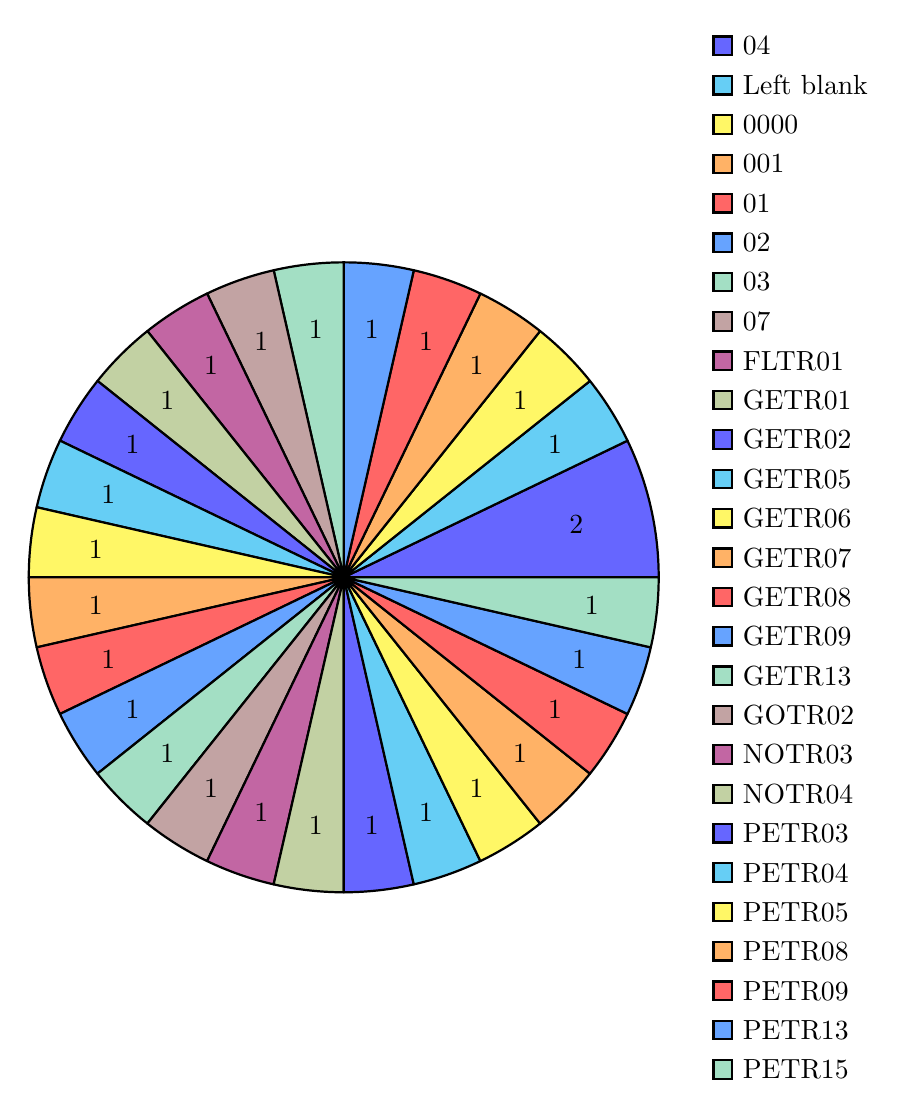
\begin{tikzpicture}
        \pie[radius=4,sum=auto,text=legend]{
            2/04,
            1/Left blank,
            1/0000,
            1/001,
            1/01,
            1/02,
            1/03,
            1/07,
            1/FLTR01,
            1/GETR01,
            1/GETR02,
            1/GETR05,
            1/GETR06,
            1/GETR07,
            1/GETR08,
            1/GETR09,
            1/GETR13,
            1/GOTR02,
            1/NOTR03,
            1/NOTR04,
            1/PETR03,
            1/PETR04,
            1/PETR05,
            1/PETR08,
            1/PETR09,
            1/PETR13,
            1/PETR15
        }
    \end{tikzpicture}
    \caption{\label{figure:q179-1}Repartition of answers for the question 'รหัสผู้ทะเบียน'.}
\end{figure}



\clearpage{}
\section{ผู้เก็บข้อมูล}

\label{sec:249}


\begin{figure}[h!]
    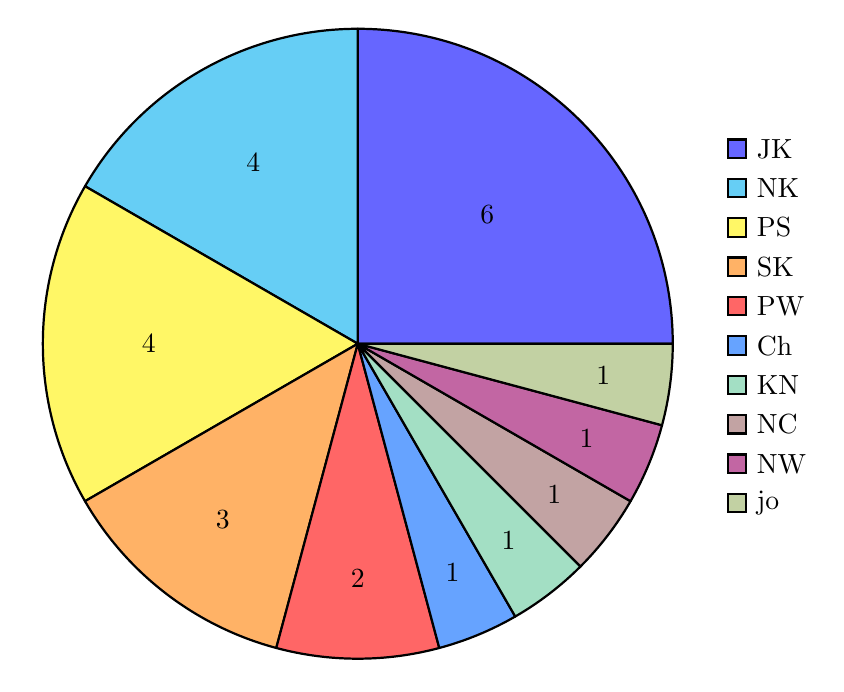
\begin{tikzpicture}
        \pie[radius=4,sum=auto,text=legend]{
            6/JK,
            4/NK,
            4/PS,
            3/SK,
            2/PW,
            1/Ch,
            1/KN,
            1/NC,
            1/NW,
            1/jo
        }
    \end{tikzpicture}
    \caption{\label{figure:q249-1}Repartition of answers for the question 'ผู้เก็บข้อมูล'.}
\end{figure}



\clearpage{}
\section{ท่านแสดงความคิดเห็นหรือร้องเรียนให้สถานบริการรับทราบทุกครั้งเมื่อมีปัญหาในการรับบริการ}

\label{sec:73}


\begin{figure}[h!]
    \begin{tikzpicture}
        \pie[radius=4,sum=auto,text=legend]{
            12/0-ไมเลย,
            7/2-ปานกลาง,
            5/Left blank,
            5/1-เลกนอย,
            3/3-มาก
        }
    \end{tikzpicture}
    \caption{\label{figure:q73-1}Repartition of answers for the question 'ท่านแสดงความคิดเห็นหรือร้องเรียนให้สถานบริการรับทราบทุกครั้งเมื่อมีปัญหาในการรับบริการ'.}
\end{figure}



\clearpage{}
\section{ท่านจัดเวลาในการดูแลสุขภาพช่องปากได้สม่ำเสมอเป็นประจำทุกวัน}

\label{sec:74}


\begin{figure}[h!]
    \begin{tikzpicture}
        \pie[radius=4,sum=auto,text=legend]{
            12/3-มาก,
            7/2-ปานกลาง,
            6/4-มากทสด,
            5/Left blank,
            2/1-เลกนอย
        }
    \end{tikzpicture}
    \caption{\label{figure:q74-1}Repartition of answers for the question 'ท่านจัดเวลาในการดูแลสุขภาพช่องปากได้สม่ำเสมอเป็นประจำทุกวัน'.}
\end{figure}



\clearpage{}
\section{ท่านอ่านฉลากเพื่อดูคุณลักษณะของผลิตภัณฑ์ดูแลสุขภาพช่องปากให้ตรงตามที่ต้องการ ก่อนซื้อทุกครั้ง}

\label{sec:75}


\begin{figure}[h!]
    \begin{tikzpicture}
        \pie[radius=4,sum=auto,text=legend]{
            11/3-มาก,
            7/4-มากทสด,
            5/Left blank,
            4/2-ปานกลาง,
            3/1-เลกนอย,
            2/0-ไมเลย
        }
    \end{tikzpicture}
    \caption{\label{figure:q75-1}Repartition of answers for the question 'ท่านอ่านฉลากเพื่อดูคุณลักษณะของผลิตภัณฑ์ดูแลสุขภาพช่องปากให้ตรงตามที่ต้องการ ก่อนซื้อทุกครั้ง'.}
\end{figure}



\clearpage{}
\section{ท่านรู้สึกอายที่ต้องอ้าปากให้หมอฟันตรวจ}

\label{sec:76}


\begin{figure}[h!]
    \begin{tikzpicture}
        \pie[radius=4,sum=auto,text=legend]{
            11/0-ไมเลย,
            6/Left blank,
            6/2-ปานกลาง,
            5/1-เลกนอย,
            2/3-มาก,
            2/4-มากทสด
        }
    \end{tikzpicture}
    \caption{\label{figure:q76-1}Repartition of answers for the question 'ท่านรู้สึกอายที่ต้องอ้าปากให้หมอฟันตรวจ'.}
\end{figure}



\clearpage{}
\section{ท่านเปรียบเทียบข้อมูลจากหลาย ๆ แหล่งทุกครั้งก่อนตัดสินใจเชื่อเสมอ}

\label{sec:77}


\begin{figure}[h!]
    \begin{tikzpicture}
        \pie[radius=4,sum=auto,text=legend]{
            11/3-มาก,
            6/Left blank,
            5/1-เลกนอย,
            5/2-ปานกลาง,
            3/0-ไมเลย,
            2/4-มากทสด
        }
    \end{tikzpicture}
    \caption{\label{figure:q77-1}Repartition of answers for the question 'ท่านเปรียบเทียบข้อมูลจากหลาย ๆ แหล่งทุกครั้งก่อนตัดสินใจเชื่อเสมอ'.}
\end{figure}



\clearpage{}
\section{เมื่อขนแปรงสีฟันบาน ท่านเปลี่ยนแปรงสีฟันทันที}

\label{sec:78}


\begin{figure}[h!]
    \begin{tikzpicture}
        \pie[radius=4,sum=auto,text=legend]{
            11/4-มากทสด,
            10/3-มาก,
            6/Left blank,
            3/2-ปานกลาง,
            1/0-ไมเลย,
            1/1-เลกนอย
        }
    \end{tikzpicture}
    \caption{\label{figure:q78-1}Repartition of answers for the question 'เมื่อขนแปรงสีฟันบาน ท่านเปลี่ยนแปรงสีฟันทันที'.}
\end{figure}



\clearpage{}
\section{ท่านตรวจสุขภาพช่องปากกับหมอฟันเป็นประจำทุกปี}

\label{sec:79}


\begin{figure}[h!]
    \begin{tikzpicture}
        \pie[radius=4,sum=auto,text=legend]{
            8/0-ไมเลย,
            7/1-เลกนอย,
            6/3-มาก,
            5/Left blank,
            3/2-ปานกลาง,
            3/4-มากทสด
        }
    \end{tikzpicture}
    \caption{\label{figure:q79-1}Repartition of answers for the question 'ท่านตรวจสุขภาพช่องปากกับหมอฟันเป็นประจำทุกปี'.}
\end{figure}



\clearpage{}
\section{ท่านสามารถเลือกผลิตภัณฑ์ที่มีคุณสมบัติเหมาะกับสภาพช่องปากตนเองได้ทุกครั้ง}

\label{sec:80}


\begin{figure}[h!]
    \begin{tikzpicture}
        \pie[radius=4,sum=auto,text=legend]{
            9/3-มาก,
            8/4-มากทสด,
            6/Left blank,
            6/2-ปานกลาง,
            2/1-เลกนอย,
            1/0-ไมเลย
        }
    \end{tikzpicture}
    \caption{\label{figure:q80-1}Repartition of answers for the question 'ท่านสามารถเลือกผลิตภัณฑ์ที่มีคุณสมบัติเหมาะกับสภาพช่องปากตนเองได้ทุกครั้ง'.}
\end{figure}



\clearpage{}
\section{ท่านสามารถแนะนำวิธีการขจัดความกลัวในการทำฟันแก่คนอื่นๆได้}

\label{sec:81}


\begin{figure}[h!]
    \begin{tikzpicture}
        \pie[radius=4,sum=auto,text=legend]{
            12/2-ปานกลาง,
            6/Left blank,
            4/0-ไมเลย,
            4/1-เลกนอย,
            4/3-มาก,
            2/4-มากทสด
        }
    \end{tikzpicture}
    \caption{\label{figure:q81-1}Repartition of answers for the question 'ท่านสามารถแนะนำวิธีการขจัดความกลัวในการทำฟันแก่คนอื่นๆได้'.}
\end{figure}



\clearpage{}
\section{ท่านตรวจสอบความถูกต้องของข้อมูลจากหลายๆแหล่งก่อนนำมาใช้ดูแลช่องปากเสมอ}

\label{sec:82}


\begin{figure}[h!]
    \begin{tikzpicture}
        \pie[radius=4,sum=auto,text=legend]{
            12/3-มาก,
            6/0-ไมเลย,
            6/2-ปานกลาง,
            5/Left blank,
            2/1-เลกนอย,
            1/4-มากทสด
        }
    \end{tikzpicture}
    \caption{\label{figure:q82-1}Repartition of answers for the question 'ท่านตรวจสอบความถูกต้องของข้อมูลจากหลายๆแหล่งก่อนนำมาใช้ดูแลช่องปากเสมอ'.}
\end{figure}



\clearpage{}
\section{คนใกล้ชิดคอยเตือนเสมอ ถ้าพบว่าท่านมีปัญหาสุขภาพช่องปาก}

\label{sec:83}


\begin{figure}[h!]
    \begin{tikzpicture}
        \pie[radius=4,sum=auto,text=legend]{
            9/2-ปานกลาง,
            6/Left blank,
            6/1-เลกนอย,
            5/0-ไมเลย,
            5/3-มาก,
            1/4-มากทสด
        }
    \end{tikzpicture}
    \caption{\label{figure:q83-1}Repartition of answers for the question 'คนใกล้ชิดคอยเตือนเสมอ ถ้าพบว่าท่านมีปัญหาสุขภาพช่องปาก'.}
\end{figure}



\clearpage{}
\section{ท่านลำบากใจในการพูดคุยปัญหากลิ่นปากกับคนอื่น ๆ}

\label{sec:84}


\begin{figure}[h!]
    \begin{tikzpicture}
        \pie[radius=4,sum=auto,text=legend]{
            8/3-มาก,
            7/1-เลกนอย,
            5/Left blank,
            5/2-ปานกลาง,
            4/0-ไมเลย,
            3/4-มากทสด
        }
    \end{tikzpicture}
    \caption{\label{figure:q84-1}Repartition of answers for the question 'ท่านลำบากใจในการพูดคุยปัญหากลิ่นปากกับคนอื่น ๆ'.}
\end{figure}



\clearpage{}
\section{ท่านรู้ว่าสิทธิประโยชน์ตามสิทธิการรักษาของท่านเป็นอย่างดี}

\label{sec:85}


\begin{figure}[h!]
    \begin{tikzpicture}
        \pie[radius=4,sum=auto,text=legend]{
            11/2-ปานกลาง,
            8/4-มากทสด,
            6/Left blank,
            5/3-มาก,
            2/1-เลกนอย
        }
    \end{tikzpicture}
    \caption{\label{figure:q85-1}Repartition of answers for the question 'ท่านรู้ว่าสิทธิประโยชน์ตามสิทธิการรักษาของท่านเป็นอย่างดี'.}
\end{figure}



\clearpage{}
\section{ท่านสามารถให้คำแนะนำการดูแลสุขภาพช่องปากแก่คนอื่น ๆด้วยความมั่นใจ}

\label{sec:86}


\begin{figure}[h!]
    \begin{tikzpicture}
        \pie[radius=4,sum=auto,text=legend]{
            13/2-ปานกลาง,
            6/1-เลกนอย,
            5/Left blank,
            4/3-มาก,
            3/0-ไมเลย,
            1/4-มากทสด
        }
    \end{tikzpicture}
    \caption{\label{figure:q86-1}Repartition of answers for the question 'ท่านสามารถให้คำแนะนำการดูแลสุขภาพช่องปากแก่คนอื่น ๆด้วยความมั่นใจ'.}
\end{figure}



\clearpage{}
\section{ท่านมีหลายช่องทางในการหาความรู้เกี่ยวกับการรักษาความสะอาดช่องปาก}

\label{sec:87}


\begin{figure}[h!]
    \begin{tikzpicture}
        \pie[radius=4,sum=auto,text=legend]{
            12/2-ปานกลาง,
            6/Left blank,
            6/3-มาก,
            5/0-ไมเลย,
            2/4-มากทสด,
            1/1-เลกนอย
        }
    \end{tikzpicture}
    \caption{\label{figure:q87-1}Repartition of answers for the question 'ท่านมีหลายช่องทางในการหาความรู้เกี่ยวกับการรักษาความสะอาดช่องปาก'.}
\end{figure}



\clearpage{}
\section{ท่านหลีกเลี่ยงการรับประทานอาหารที่อาจทำร้ายเหงือกและฟันเสมอ}

\label{sec:88}


\begin{figure}[h!]
    \begin{tikzpicture}
        \pie[radius=4,sum=auto,text=legend]{
            12/3-มาก,
            8/2-ปานกลาง,
            6/Left blank,
            5/1-เลกนอย,
            1/4-มากทสด
        }
    \end{tikzpicture}
    \caption{\label{figure:q88-1}Repartition of answers for the question 'ท่านหลีกเลี่ยงการรับประทานอาหารที่อาจทำร้ายเหงือกและฟันเสมอ'.}
\end{figure}



\clearpage{}
\section{ท่านสามารถนำสิ่งที่หมอฟันแนะนำมาปฏิบัติในชีวิตประจำวันได้อย่างถูกต้องครบถ้วน}

\label{sec:89}


\begin{figure}[h!]
    \begin{tikzpicture}
        \pie[radius=4,sum=auto,text=legend]{
            11/2-ปานกลาง,
            9/3-มาก,
            6/Left blank,
            3/1-เลกนอย,
            2/0-ไมเลย,
            1/4-มากทสด
        }
    \end{tikzpicture}
    \caption{\label{figure:q89-1}Repartition of answers for the question 'ท่านสามารถนำสิ่งที่หมอฟันแนะนำมาปฏิบัติในชีวิตประจำวันได้อย่างถูกต้องครบถ้วน'.}
\end{figure}



\clearpage{}
\section{ท่านสามารถจัดการค่าใช้จ่ายในการรักษาปัญหาสุขภาพช่องปากได้ทุกครั้ง}

\label{sec:90}


\begin{figure}[h!]
    \begin{tikzpicture}
        \pie[radius=4,sum=auto,text=legend]{
            10/2-ปานกลาง,
            8/3-มาก,
            7/Left blank,
            5/1-เลกนอย,
            2/4-มากทสด
        }
    \end{tikzpicture}
    \caption{\label{figure:q90-1}Repartition of answers for the question 'ท่านสามารถจัดการค่าใช้จ่ายในการรักษาปัญหาสุขภาพช่องปากได้ทุกครั้ง'.}
\end{figure}



\clearpage{}
\section{ตัวท่านมีบทบาทสำคัญที่สุดในการดูแลรักษาสุขภาพช่องปาก}

\label{sec:91}


\begin{figure}[h!]
    \begin{tikzpicture}
        \pie[radius=4,sum=auto,text=legend]{
            15/3-มาก,
            6/Left blank,
            4/2-ปานกลาง,
            3/4-มากทสด,
            2/0-ไมเลย,
            2/1-เลกนอย
        }
    \end{tikzpicture}
    \caption{\label{figure:q91-1}Repartition of answers for the question 'ตัวท่านมีบทบาทสำคัญที่สุดในการดูแลรักษาสุขภาพช่องปาก'.}
\end{figure}



\clearpage{}
\section{ท่านรู้สึกไม่อยากพูดคุยกับหมอฟันขณะทำฟัน}

\label{sec:92}


\begin{figure}[h!]
    \begin{tikzpicture}
        \pie[radius=4,sum=auto,text=legend]{
            9/3-มาก,
            6/Left blank,
            6/1-เลกนอย,
            5/0-ไมเลย,
            5/2-ปานกลาง,
            1/4-มากทสด
        }
    \end{tikzpicture}
    \caption{\label{figure:q92-1}Repartition of answers for the question 'ท่านรู้สึกไม่อยากพูดคุยกับหมอฟันขณะทำฟัน'.}
\end{figure}



\clearpage{}
\section{ท่านเข้าใจทุกอย่างที่หมอฟันอธิบายเกี่ยวกับสุขภาพช่องปากของท่าน}

\label{sec:93}


\begin{figure}[h!]
    \begin{tikzpicture}
        \pie[radius=4,sum=auto,text=legend]{
            11/3-มาก,
            7/Left blank,
            7/2-ปานกลาง,
            5/4-มากทสด,
            1/0-ไมเลย,
            1/1-เลกนอย
        }
    \end{tikzpicture}
    \caption{\label{figure:q93-1}Repartition of answers for the question 'ท่านเข้าใจทุกอย่างที่หมอฟันอธิบายเกี่ยวกับสุขภาพช่องปากของท่าน'.}
\end{figure}



\clearpage{}
\section{ท่านซักถามข้อสงสัยต่างๆกับหมอฟันจนเข้าใจดีเกี่ยวกับปัญหาสุขภาพช่องปาก}

\label{sec:94}


\begin{figure}[h!]
    \begin{tikzpicture}
        \pie[radius=4,sum=auto,text=legend]{
            15/3-มาก,
            7/Left blank,
            6/2-ปานกลาง,
            2/0-ไมเลย,
            2/1-เลกนอย
        }
    \end{tikzpicture}
    \caption{\label{figure:q94-1}Repartition of answers for the question 'ท่านซักถามข้อสงสัยต่างๆกับหมอฟันจนเข้าใจดีเกี่ยวกับปัญหาสุขภาพช่องปาก'.}
\end{figure}



\clearpage{}
\section{ท่านใช้ไหมขัดฟันทำความสะอาดได้ทุกซอกฟัน วันละ 1 ครั้ง}

\label{sec:95}


\begin{figure}[h!]
    \begin{tikzpicture}
        \pie[radius=4,sum=auto,text=legend]{
            17/0-ไมเลย,
            7/Left blank,
            4/1-เลกนอย,
            3/2-ปานกลาง,
            1/4-มากทสด
        }
    \end{tikzpicture}
    \caption{\label{figure:q95-1}Repartition of answers for the question 'ท่านใช้ไหมขัดฟันทำความสะอาดได้ทุกซอกฟัน วันละ 1 ครั้ง'.}
\end{figure}



\clearpage{}
\section{ถ้าท่านมารับบริการทำฟัน ท่านมีส่วนร่วมตัดสินใจเลือกการรักษาทุกครั้ง}

\label{sec:96}


\begin{figure}[h!]
    \begin{tikzpicture}
        \pie[radius=4,sum=auto,text=legend]{
            9/3-มาก,
            7/Left blank,
            6/2-ปานกลาง,
            6/4-มากทสด,
            3/1-เลกนอย,
            1/0-ไมเลย
        }
    \end{tikzpicture}
    \caption{\label{figure:q96-1}Repartition of answers for the question 'ถ้าท่านมารับบริการทำฟัน ท่านมีส่วนร่วมตัดสินใจเลือกการรักษาทุกครั้ง'.}
\end{figure}



\clearpage{}
\section{ท่านสามารถตัดสินใจได้ว่าเมื่อไรควรไปพบหมอฟัน}

\label{sec:97}


\begin{figure}[h!]
    \begin{tikzpicture}
        \pie[radius=4,sum=auto,text=legend]{
            14/3-มาก,
            7/Left blank,
            5/2-ปานกลาง,
            3/0-ไมเลย,
            3/4-มากทสด
        }
    \end{tikzpicture}
    \caption{\label{figure:q97-1}Repartition of answers for the question 'ท่านสามารถตัดสินใจได้ว่าเมื่อไรควรไปพบหมอฟัน'.}
\end{figure}



\clearpage{}
\section{ท่านเข้าใจเนื้อหาบนฉลากของผลิตภัณฑ์ดูแลสุขภาพช่องปากได้เป็นอย่างดี}

\label{sec:98}


\begin{figure}[h!]
    \begin{tikzpicture}
        \pie[radius=4,sum=auto,text=legend]{
            11/3-มาก,
            7/Left blank,
            7/4-มากทสด,
            6/2-ปานกลาง,
            1/1-เลกนอย
        }
    \end{tikzpicture}
    \caption{\label{figure:q98-1}Repartition of answers for the question 'ท่านเข้าใจเนื้อหาบนฉลากของผลิตภัณฑ์ดูแลสุขภาพช่องปากได้เป็นอย่างดี'.}
\end{figure}



\clearpage{}
\section{ท่านเลือกสถานบริการที่แก้ปัญหาสุขภาพช่องปากได้ตรงตามความต้องการของท่านทุกครั้ง}

\label{sec:99}


\begin{figure}[h!]
    \begin{tikzpicture}
        \pie[radius=4,sum=auto,text=legend]{
            10/3-มาก,
            7/Left blank,
            7/2-ปานกลาง,
            6/4-มากทสด,
            1/0-ไมเลย,
            1/1-เลกนอย
        }
    \end{tikzpicture}
    \caption{\label{figure:q99-1}Repartition of answers for the question 'ท่านเลือกสถานบริการที่แก้ปัญหาสุขภาพช่องปากได้ตรงตามความต้องการของท่านทุกครั้ง'.}
\end{figure}



\clearpage{}
\section{ท่านรู้ลักษณะที่ดีของผลิตภัณฑ์แต่ละชนิดในการดูแลสุขภาพช่องปาก}

\label{sec:100}


\begin{figure}[h!]
    \begin{tikzpicture}
        \pie[radius=4,sum=auto,text=legend]{
            13/2-ปานกลาง,
            8/3-มาก,
            7/Left blank,
            3/1-เลกนอย,
            1/4-มากทสด
        }
    \end{tikzpicture}
    \caption{\label{figure:q100-1}Repartition of answers for the question 'ท่านรู้ลักษณะที่ดีของผลิตภัณฑ์แต่ละชนิดในการดูแลสุขภาพช่องปาก'.}
\end{figure}



\clearpage{}
\section{ท่านรู้ว่าถ้าสุขภาพช่องปากไม่ดี อาจทำให้ป่วยเป็นโรคอื่นๆได้}

\label{sec:101}


\begin{figure}[h!]
    \begin{tikzpicture}
        \pie[radius=4,sum=auto,text=legend]{
            10/3-มาก,
            8/2-ปานกลาง,
            7/Left blank,
            3/0-ไมเลย,
            2/1-เลกนอย,
            2/4-มากทสด
        }
    \end{tikzpicture}
    \caption{\label{figure:q101-1}Repartition of answers for the question 'ท่านรู้ว่าถ้าสุขภาพช่องปากไม่ดี อาจทำให้ป่วยเป็นโรคอื่นๆได้'.}
\end{figure}



\clearpage{}
\section{ท่านใช้สิทธิการรักษาของตนเองทุกครั้งที่ไปรับบริการ}

\label{sec:102}


\begin{figure}[h!]
    \begin{tikzpicture}
        \pie[radius=4,sum=auto,text=legend]{
            10/4-มากทสด,
            8/3-มาก,
            7/Left blank,
            4/2-ปานกลาง,
            2/0-ไมเลย,
            1/1-เลกนอย
        }
    \end{tikzpicture}
    \caption{\label{figure:q102-1}Repartition of answers for the question 'ท่านใช้สิทธิการรักษาของตนเองทุกครั้งที่ไปรับบริการ'.}
\end{figure}



\clearpage{}
\section{ท่านตรวจสอบความสะอาดช่องปากหลังทำความสะอาดทุกครั้ง}

\label{sec:103}


\begin{figure}[h!]
    \begin{tikzpicture}
        \pie[radius=4,sum=auto,text=legend]{
            8/2-ปานกลาง,
            8/3-มาก,
            7/Left blank,
            4/1-เลกนอย,
            4/4-มากทสด,
            1/0-ไมเลย
        }
    \end{tikzpicture}
    \caption{\label{figure:q103-1}Repartition of answers for the question 'ท่านตรวจสอบความสะอาดช่องปากหลังทำความสะอาดทุกครั้ง'.}
\end{figure}



\clearpage{}
\section{ท่านสามารถค้นหาข้อมูลที่ถูกต้องได้ตามที่ต้องการเสมอเกี่ยวกับการดูแลสุขภาพช่องปาก}

\label{sec:104}


\begin{figure}[h!]
    \begin{tikzpicture}
        \pie[radius=4,sum=auto,text=legend]{
            8/2-ปานกลาง,
            8/3-มาก,
            7/Left blank,
            4/0-ไมเลย,
            4/1-เลกนอย,
            1/4-มากทสด
        }
    \end{tikzpicture}
    \caption{\label{figure:q104-1}Repartition of answers for the question 'ท่านสามารถค้นหาข้อมูลที่ถูกต้องได้ตามที่ต้องการเสมอเกี่ยวกับการดูแลสุขภาพช่องปาก'.}
\end{figure}



\clearpage{}
\section{ท่านเข้าใจข้อมูลเกี่ยวกับการรักษาสุขภาพช่องปากจากสื่อต่างๆได้ดีพอที่จะนำไปใช้ได้}

\label{sec:105}


\begin{figure}[h!]
    \begin{tikzpicture}
        \pie[radius=4,sum=auto,text=legend]{
            8/3-มาก,
            7/2-ปานกลาง,
            6/Left blank,
            6/1-เลกนอย,
            3/4-มากทสด,
            2/0-ไมเลย
        }
    \end{tikzpicture}
    \caption{\label{figure:q105-1}Repartition of answers for the question 'ท่านเข้าใจข้อมูลเกี่ยวกับการรักษาสุขภาพช่องปากจากสื่อต่างๆได้ดีพอที่จะนำไปใช้ได้'.}
\end{figure}



\clearpage{}
\section{ท่านรู้ดีว่าสุขภาพช่องปากของตนเองเป็นอย่างไร}

\label{sec:106}


\begin{figure}[h!]
    \begin{tikzpicture}
        \pie[radius=4,sum=auto,text=legend]{
            13/3-มาก,
            7/Left blank,
            7/2-ปานกลาง,
            4/1-เลกนอย,
            1/0-ไมเลย
        }
    \end{tikzpicture}
    \caption{\label{figure:q106-1}Repartition of answers for the question 'ท่านรู้ดีว่าสุขภาพช่องปากของตนเองเป็นอย่างไร'.}
\end{figure}



\clearpage{}
\section{ท่านถามค่าใช้จ่ายในการรักษากับหมอฟันทุกครั้งก่อนเริ่มการรักษา}

\label{sec:107}


\begin{figure}[h!]
    \begin{tikzpicture}
        \pie[radius=4,sum=auto,text=legend]{
            9/4-มากทสด,
            7/Left blank,
            5/2-ปานกลาง,
            5/3-มาก,
            4/0-ไมเลย,
            2/1-เลกนอย
        }
    \end{tikzpicture}
    \caption{\label{figure:q107-1}Repartition of answers for the question 'ท่านถามค่าใช้จ่ายในการรักษากับหมอฟันทุกครั้งก่อนเริ่มการรักษา'.}
\end{figure}



\clearpage{}
\section{ท่านคิดว่าใช้น้ำยาบ้วนปากทดแทนการแปรงฟันได้}

\label{sec:108}


\begin{figure}[h!]
    \begin{tikzpicture}
        \pie[radius=4,sum=auto,text=legend]{
            9/2-ปานกลาง,
            8/1-เลกนอย,
            7/Left blank,
            6/0-ไมเลย,
            2/3-มาก
        }
    \end{tikzpicture}
    \caption{\label{figure:q108-1}Repartition of answers for the question 'ท่านคิดว่าใช้น้ำยาบ้วนปากทดแทนการแปรงฟันได้'.}
\end{figure}



\clearpage{}
\section{ท่านสามารถซักถามข้อสงสัยเกี่ยวกับสิทธิการรักษาจากเจ้าหน้าที่}

\label{sec:109}


\begin{figure}[h!]
    \begin{tikzpicture}
        \pie[radius=4,sum=auto,text=legend]{
            13/3-มาก,
            7/Left blank,
            5/4-มากทสด,
            4/2-ปานกลาง,
            2/0-ไมเลย,
            1/1-เลกนอย
        }
    \end{tikzpicture}
    \caption{\label{figure:q109-1}Repartition of answers for the question 'ท่านสามารถซักถามข้อสงสัยเกี่ยวกับสิทธิการรักษาจากเจ้าหน้าที่'.}
\end{figure}



\clearpage{}
\section{ฉันดูแลสุขภาพช่องปากได้เป็นอย่างดีทำให้มั่นใจในการยิ้ม พูดคุยกับคนอื่นๆ}

\label{sec:110}


\begin{figure}[h!]
    \begin{tikzpicture}
        \pie[radius=4,sum=auto,text=legend]{
            15/3-มาก,
            8/2-ปานกลาง,
            7/Left blank,
            2/1-เลกนอย
        }
    \end{tikzpicture}
    \caption{\label{figure:q110-1}Repartition of answers for the question 'ฉันดูแลสุขภาพช่องปากได้เป็นอย่างดีทำให้มั่นใจในการยิ้ม พูดคุยกับคนอื่นๆ'.}
\end{figure}



\clearpage{}
\section{ท่านสามารถแนะนำคนอื่น ๆ ในการเลือกผลิตภัณฑ์ดูแลสุขภาพช่องปากที่เหมาะสมได้}

\label{sec:111}


\begin{figure}[h!]
    \begin{tikzpicture}
        \pie[radius=4,sum=auto,text=legend]{
            10/2-ปานกลาง,
            6/Left blank,
            6/3-มาก,
            5/0-ไมเลย,
            4/1-เลกนอย,
            1/4-มากทสด
        }
    \end{tikzpicture}
    \caption{\label{figure:q111-1}Repartition of answers for the question 'ท่านสามารถแนะนำคนอื่น ๆ ในการเลือกผลิตภัณฑ์ดูแลสุขภาพช่องปากที่เหมาะสมได้'.}
\end{figure}



\clearpage{}
\section{การทำงานของท่านเป็นอุปสรรคต่อการดูแลสุขภาพช่องปาก}

\label{sec:112}


\begin{figure}[h!]
    \begin{tikzpicture}
        \pie[radius=4,sum=auto,text=legend]{
            14/0-ไมเลย,
            7/Left blank,
            6/1-เลกนอย,
            4/2-ปานกลาง,
            1/3-มาก
        }
    \end{tikzpicture}
    \caption{\label{figure:q112-1}Repartition of answers for the question 'การทำงานของท่านเป็นอุปสรรคต่อการดูแลสุขภาพช่องปาก'.}
\end{figure}



\clearpage{}
\section{ท่านสามารถหาข้อมูลเกี่ยวกับการให้บริการทันตกรรมของโรงพยาบาล/ คลินิกทำฟันได้}

\label{sec:113}


\begin{figure}[h!]
    \begin{tikzpicture}
        \pie[radius=4,sum=auto,text=legend]{
            12/3-มาก,
            7/Left blank,
            6/2-ปานกลาง,
            4/1-เลกนอย,
            2/0-ไมเลย,
            1/4-มากทสด
        }
    \end{tikzpicture}
    \caption{\label{figure:q113-1}Repartition of answers for the question 'ท่านสามารถหาข้อมูลเกี่ยวกับการให้บริการทันตกรรมของโรงพยาบาล/ คลินิกทำฟันได้'.}
\end{figure}



\clearpage{}
\section{สมาชิกในครอบครัวท่าน ใส่ใจดูแลสุขภาพช่องปากให้กันและกันอย่างสม่ำเสมอ}

\label{sec:114}


\begin{figure}[h!]
    \begin{tikzpicture}
        \pie[radius=4,sum=auto,text=legend]{
            12/3-มาก,
            8/2-ปานกลาง,
            7/Left blank,
            3/4-มากทสด,
            1/0-ไมเลย,
            1/1-เลกนอย
        }
    \end{tikzpicture}
    \caption{\label{figure:q114-1}Repartition of answers for the question 'สมาชิกในครอบครัวท่าน ใส่ใจดูแลสุขภาพช่องปากให้กันและกันอย่างสม่ำเสมอ'.}
\end{figure}



\clearpage{}
\section{ท่านอ่านฉลากในการเลือกยาสีฟันที่มีส่วนผสมของฟลูออไรด์ใช้เสมอ}

\label{sec:115}


\begin{figure}[h!]
    \begin{tikzpicture}
        \pie[radius=4,sum=auto,text=legend]{
            10/3-มาก,
            7/Left blank,
            6/4-มากทสด,
            5/2-ปานกลาง,
            2/0-ไมเลย,
            2/1-เลกนอย
        }
    \end{tikzpicture}
    \caption{\label{figure:q115-1}Repartition of answers for the question 'ท่านอ่านฉลากในการเลือกยาสีฟันที่มีส่วนผสมของฟลูออไรด์ใช้เสมอ'.}
\end{figure}



\clearpage{}
\section{ท่านสามารถหาข้อมูลที่ต้องการได้ทุกครั้งเกี่ยวกับการดูแลความสะอาดช่องปาก}

\label{sec:116}


\begin{figure}[h!]
    \begin{tikzpicture}
        \pie[radius=4,sum=auto,text=legend]{
            9/3-มาก,
            8/2-ปานกลาง,
            6/Left blank,
            5/1-เลกนอย,
            3/4-มากทสด,
            1/0-ไมเลย
        }
    \end{tikzpicture}
    \caption{\label{figure:q116-1}Repartition of answers for the question 'ท่านสามารถหาข้อมูลที่ต้องการได้ทุกครั้งเกี่ยวกับการดูแลความสะอาดช่องปาก'.}
\end{figure}



\clearpage{}
\section{ท่านกล้าบอกหมอฟันว่าท่านกลัวการทำฟัน}

\label{sec:117}


\begin{figure}[h!]
    \begin{tikzpicture}
        \pie[radius=4,sum=auto,text=legend]{
            8/2-ปานกลาง,
            8/3-มาก,
            7/Left blank,
            5/0-ไมเลย,
            4/4-มากทสด
        }
    \end{tikzpicture}
    \caption{\label{figure:q117-1}Repartition of answers for the question 'ท่านกล้าบอกหมอฟันว่าท่านกลัวการทำฟัน'.}
\end{figure}



\clearpage{}
\section{ท่านแปรงฟันทั่วทุกซี่ วันละ 2 ครั้ง ครั้งละ อย่างน้อย 2 นาที ด้วยยาสีฟันที่มีฟลูออไรด์ทุกครั้ง}

\label{sec:118}


\begin{figure}[h!]
    \begin{tikzpicture}
        \pie[radius=4,sum=auto,text=legend]{
            10/2-ปานกลาง,
            9/3-มาก,
            7/Left blank,
            5/4-มากทสด,
            1/1-เลกนอย
        }
    \end{tikzpicture}
    \caption{\label{figure:q118-1}Repartition of answers for the question 'ท่านแปรงฟันทั่วทุกซี่ วันละ 2 ครั้ง ครั้งละ อย่างน้อย 2 นาที ด้วยยาสีฟันที่มีฟลูออไรด์ทุกครั้ง'.}
\end{figure}



\clearpage{}
\section{ท่านรู้สึกว่ายากที่จะเข้าใจข้อมูลเกี่ยวกับสุขภาพช่องปาก}

\label{sec:119}


\begin{figure}[h!]
    \begin{tikzpicture}
        \pie[radius=4,sum=auto,text=legend]{
            11/2-ปานกลาง,
            7/Left blank,
            7/3-มาก,
            4/1-เลกนอย,
            2/4-มากทสด,
            1/0-ไมเลย
        }
    \end{tikzpicture}
    \caption{\label{figure:q119-1}Repartition of answers for the question 'ท่านรู้สึกว่ายากที่จะเข้าใจข้อมูลเกี่ยวกับสุขภาพช่องปาก'.}
\end{figure}



\clearpage{}
\section{ท่านสามารถขอความช่วยเหลือในการดูแลสุขภาพช่องปาก จากครอบครัว เพื่อน หรือคนใกล้ชิด ยามที่ท่านต้องการ}

\label{sec:120}


\begin{figure}[h!]
    \begin{tikzpicture}
        \pie[radius=4,sum=auto,text=legend]{
            12/3-มาก,
            7/Left blank,
            7/2-ปานกลาง,
            4/1-เลกนอย,
            2/4-มากทสด
        }
    \end{tikzpicture}
    \caption{\label{figure:q120-1}Repartition of answers for the question 'ท่านสามารถขอความช่วยเหลือในการดูแลสุขภาพช่องปาก จากครอบครัว เพื่อน หรือคนใกล้ชิด ยามที่ท่านต้องการ'.}
\end{figure}



\clearpage{}
\section{ความกลัวไม่มีผลต่อการตัดสินใจไปทำฟัน}

\label{sec:121}


\begin{figure}[h!]
    \begin{tikzpicture}
        \pie[radius=4,sum=auto,text=legend]{
            7/Left blank,
            7/0-ไมเลย,
            6/3-มาก,
            5/2-ปานกลาง,
            4/1-เลกนอย,
            3/4-มากทสด
        }
    \end{tikzpicture}
    \caption{\label{figure:q121-1}Repartition of answers for the question 'ความกลัวไม่มีผลต่อการตัดสินใจไปทำฟัน'.}
\end{figure}



\clearpage{}
\section{ท่านไปหาหมอฟัน เมื่อมีอาการรุนแรงจนทนไม่ไหวทุกครั้ง}

\label{sec:122}


\begin{figure}[h!]
    \begin{tikzpicture}
        \pie[radius=4,sum=auto,text=legend]{
            7/Left blank,
            7/3-มาก,
            6/1-เลกนอย,
            6/4-มากทสด,
            4/0-ไมเลย,
            2/2-ปานกลาง
        }
    \end{tikzpicture}
    \caption{\label{figure:q122-1}Repartition of answers for the question 'ท่านไปหาหมอฟัน เมื่อมีอาการรุนแรงจนทนไม่ไหวทุกครั้ง'.}
\end{figure}



\clearpage{}
\section{ท่านค้นหาข้อมูลจากหลายๆแหล่งเสมอเกี่ยวกับวิธีการดูแลสุขภาพช่องปาก}

\label{sec:123}


\begin{figure}[h!]
    \begin{tikzpicture}
        \pie[radius=4,sum=auto,text=legend]{
            11/2-ปานกลาง,
            7/Left blank,
            6/3-มาก,
            5/0-ไมเลย,
            3/1-เลกนอย
        }
    \end{tikzpicture}
    \caption{\label{figure:q123-1}Repartition of answers for the question 'ท่านค้นหาข้อมูลจากหลายๆแหล่งเสมอเกี่ยวกับวิธีการดูแลสุขภาพช่องปาก'.}
\end{figure}



\clearpage{}
\section{ท่านรู้ว่ามีบริการด้านทันตกรรมอะไรบ้าง ใกล้ที่พักอาศัย}

\label{sec:124}


\begin{figure}[h!]
    \begin{tikzpicture}
        \pie[radius=4,sum=auto,text=legend]{
            12/2-ปานกลาง,
            11/3-มาก,
            7/Left blank,
            1/1-เลกนอย,
            1/4-มากทสด
        }
    \end{tikzpicture}
    \caption{\label{figure:q124-1}Repartition of answers for the question 'ท่านรู้ว่ามีบริการด้านทันตกรรมอะไรบ้าง ใกล้ที่พักอาศัย'.}
\end{figure}



\clearpage{}
\section{แม้จะรู้สึกกลัวการทำฟัน แต่ท่านสามารถมารับการรักษาทุกครั้ง}

\label{sec:125}


\begin{figure}[h!]
    \begin{tikzpicture}
        \pie[radius=4,sum=auto,text=legend]{
            9/4-มากทสด,
            7/Left blank,
            7/2-ปานกลาง,
            7/3-มาก,
            2/1-เลกนอย
        }
    \end{tikzpicture}
    \caption{\label{figure:q125-1}Repartition of answers for the question 'แม้จะรู้สึกกลัวการทำฟัน แต่ท่านสามารถมารับการรักษาทุกครั้ง'.}
\end{figure}



\clearpage{}
\section{ท่านกล้าซักถามขั้นตอนการรักษาหรือปัญหาที่จะเกิดขึ้นก่อนรับการรักษา}

\label{sec:126}


\begin{figure}[h!]
    \begin{tikzpicture}
        \pie[radius=4,sum=auto,text=legend]{
            9/3-มาก,
            7/Left blank,
            5/0-ไมเลย,
            5/4-มากทสด,
            4/1-เลกนอย,
            2/2-ปานกลาง
        }
    \end{tikzpicture}
    \caption{\label{figure:q126-1}Repartition of answers for the question 'ท่านกล้าซักถามขั้นตอนการรักษาหรือปัญหาที่จะเกิดขึ้นก่อนรับการรักษา'.}
\end{figure}



\clearpage{}
\section{ท่านสามารถบอกได้ว่าอะไรเป็นเหตุอาจทำให้ท่านมีสุขภาพช่องปากไม่ดี}

\label{sec:127}


\begin{figure}[h!]
    \begin{tikzpicture}
        \pie[radius=4,sum=auto,text=legend]{
            7/Left blank,
            7/2-ปานกลาง,
            7/3-มาก,
            5/1-เลกนอย,
            4/0-ไมเลย,
            2/4-มากทสด
        }
    \end{tikzpicture}
    \caption{\label{figure:q127-1}Repartition of answers for the question 'ท่านสามารถบอกได้ว่าอะไรเป็นเหตุอาจทำให้ท่านมีสุขภาพช่องปากไม่ดี'.}
\end{figure}



\clearpage{}
\section{ท่านเลือกใช้บริการรักษาสุขภาพช่องปากโดยไม่กระทบเวลาการทำงานของท่าน}

\label{sec:128}


\begin{figure}[h!]
    \begin{tikzpicture}
        \pie[radius=4,sum=auto,text=legend]{
            7/Left blank,
            6/0-ไมเลย,
            6/3-มาก,
            5/4-มากทสด,
            4/1-เลกนอย,
            4/2-ปานกลาง
        }
    \end{tikzpicture}
    \caption{\label{figure:q128-1}Repartition of answers for the question 'ท่านเลือกใช้บริการรักษาสุขภาพช่องปากโดยไม่กระทบเวลาการทำงานของท่าน'.}
\end{figure}



\clearpage{}
\section{ท่านดูแลสุขภาพช่องปากอย่างเคร่งครัด เพื่อไม่ให้เกิดปัญหามากระทบการดำเนินชีวิตประจำวัน}

\label{sec:129}


\begin{figure}[h!]
    \begin{tikzpicture}
        \pie[radius=4,sum=auto,text=legend]{
            9/3-มาก,
            7/2-ปานกลาง,
            6/Left blank,
            5/4-มากทสด,
            4/1-เลกนอย,
            1/0-ไมเลย
        }
    \end{tikzpicture}
    \caption{\label{figure:q129-1}Repartition of answers for the question 'ท่านดูแลสุขภาพช่องปากอย่างเคร่งครัด เพื่อไม่ให้เกิดปัญหามากระทบการดำเนินชีวิตประจำวัน'.}
\end{figure}



\end{document}
